\subsection{DIAGRAMS EXPRESSING ASSOCIATIVITY AND COMMUTATIVITY}

Let A be a commutative ring and E an A-module; being given a bilinear mapping of \(E \times E\) into E is equivalent to being given an A-linear mapping:

\[
m: \mathbf {E} \otimes_ {\mathbf {A}} \mathbf {E} \rightarrow \mathbf {E}
\]

(II, §3, no. 5). An A-algebra structure on E is therefore defined by giving an A-module structure on E and an A-linear mapping of E \(\otimes_{\mathbf{A}}\) E into E.

Let \(E'\) be another A-algebra and \(m': E' \otimes_{A} E' \to E'\) the A-linear mapping defining the multiplication of \(E'\) . A mapping \(f: E \to E'\) is an A-algebra homomorphism if and only if \(f\) is a mapping rendering commutative the diagram

\[
\begin{array}{c} \mathrm{E} \otimes_ {\mathrm{A}} \mathrm{E} \xrightarrow {f \otimes f} \mathrm{E} ^ {\prime} \otimes_ {\mathrm{A}} \mathrm{E} ^ {\prime} \\ m \Biggl \downarrow \\ \mathrm{E} \xrightarrow {f} \mathrm{E} ^ {\prime} \end{array}
\]

For an A-algebra E to be associative, it is necessary and sufficient (taking account of the associativity of tensor products, cf.~II, § 3, no. 8) that the diagram of A-linear mappings

\[
\begin{array}{c} \mathrm{E} \otimes_ {\mathrm{A}} \mathrm{E} \otimes_ {\mathrm{A}} \mathrm{E} \xrightarrow {m \otimes 1 _ {\mathrm{E}}} \mathrm{E} \otimes_ {\mathrm{A}} \mathrm{E} \\ \downarrow^ {1 _ {\mathrm{E}} \otimes m} \\ \mathrm{E} \otimes_ {\mathrm{A}} \mathrm{E} \xrightarrow {m} \mathrm{E} \end{array}
\]

be commutative. Similarly, for the A-algebra E to be commutative, it is necessary and sufficient that the diagram of A-linear mappings

\[
\begin{array}{c} \mathrm{E} \otimes_ {\mathrm{A}} \mathrm{E} \xrightarrow {\sigma} \mathrm{E} \otimes_ {\mathrm{A}} \mathrm{E} \\ \Biggl \downarrow m \Biggl \downarrow m \\ \mathrm{E} \end{array}
\]

be commutative, where \(\sigma\) denotes the canonical A-linear mapping defined by \(\sigma(x \otimes y) = y \otimes x\) for \(x \in \mathbf{E}\) , \(y \in \mathbf{E}\) (II, § 3, no. 1, Corollary 2 to Proposition 1).

For all \(c \in \mathbf{E}\) , let \(\eta_c\) denote the A-linear mapping of \(\mathbf{A}\) into \(\mathbf{E}\) defined by the condition \(\eta_c(1) = c\) . For \(c\) to be a unit element of \(\mathbf{E}\) , it is necessary and sufficient that the two diagrams

\pandocbounded{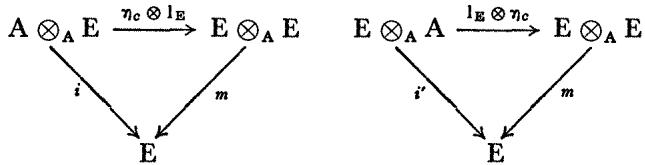
\includegraphics[keepaspectratio]{images/part003_ee0531f1.jpg}}

be commutative (i and i' denoting the canonical isomorphisms (II, §3, no. 4, Proposition 4)).

Let E be an A-algebra with unit element e and let \(\eta = \eta_{e}\) (also denoted by \(\eta_{E}\) ); then \(\eta(\alpha\beta) = \eta(\alpha)\eta(\beta) = \alpha\eta(\beta)\) , for by (2) (no. 1),

\[
(\alpha e) (\beta e) = (\alpha \beta) e = \alpha (\beta e);
\]

hence \(\eta\) is an A-algebra homomorphism. Observe that the A-module structure on E can be defined using \(\eta\) , for

\[
\alpha x = \eta (\alpha). x \quad \text { for } \alpha \in \mathrm{A}, x \in \mathrm{E}\tag{3}
\]

(where, on the right hand side, multiplication is in E). The image of the homomorphism \(\eta\) is a subalgebra of E whose elements commute with all those of E. The kernel of the homomorphism \(\eta\) is the annihilator of the element \(e\) of the A-module E; by (3), it is also the annihilator of the A-module E (II, § 1, no. 12).

When the algebra E is unital and associative, \(\eta\) is a ring homomorphism. Conversely, let \(\rho:A\to B\) be a ring homomorphism such that the image \(\rho(A)\) is contained in the centre of B, assuming also that the ring A is commutative; then an A-algebra structure is defined on B which is associative and unital, by writing (cf.~(3))

\[
\lambda x = \rho (\lambda). x \quad \text { for } \lambda \in \mathbf {A}, x \in \mathbf {E}.
\]

